\section{Introduction}\label{sec:intro}

Double reading in radiology pays off when the second reader's errors differ from the first reader's \cite{taylor2008double,geijer2018double,kurvers2016pooling}. Medical multi-agent systems use role prompts and multiagent debate to coordinate instances of one model \cite{kim2024mdagents,tang2024medagents,du2024debate,kim2026scaling}. These agents share the same model weights, including the vision encoder and language model.

We ask how many independent readings a multi-agent system of one VLM provides, and where its shared errors come from. We evaluate four proprietary and five open-weight VLMs on VQA-RAD, SLAKE, and MedXpertQA-MM, with single-agent and self-consistency baselines alongside Independent and Decentralized multi-agent systems (MAS). We measure error correlation $\phi$ and the effective number of independent agents, $N_{\mathrm{eff}}$ \cite{kish1965survey}, to quantify the return from majority voting (\cref{fig:teaser}). Controlled manipulations vary the image and what agents share. Code and data will be released.

\begin{figure}[t]
\centering
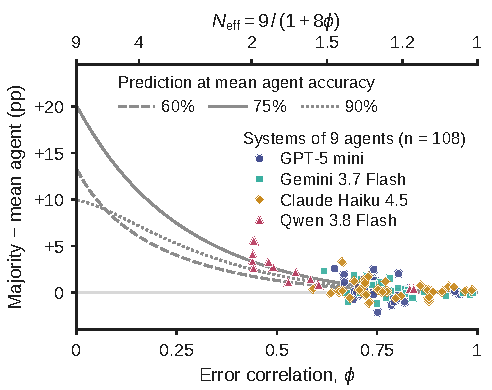
\includegraphics[width=\linewidth]{figures/fig1_teaser_col.pdf}
\caption{\textbf{The benefit of majority voting depends on error correlation.} Majority minus mean agent accuracy versus $\phi$ for $108$ systems of $9$ agents on yes/no items. Gray curves: beta-binomial predictions at mean agent accuracy $60\%$ (dashed), $75\%$ (solid), and $90\%$ (dotted). Top axis: $N_{\mathrm{eff}}=9/(1+8\phi)$. Blue circles: GPT-5 mini; teal squares: Gemini 3.7 Flash; amber diamonds: Claude Haiku 4.5; rose triangles: Qwen 3.8 Flash.}
\label{fig:teaser}
\end{figure}

\begin{itemize}
\item \textbf{Aggregation arithmetic.} Mean agent accuracy and error correlation predict every system's majority accuracy under a beta-binomial model on yes/no items (prediction-error SD: $0.84$~pp). Nine agents of one VLM in the Independent MAS provide $1.17$ to $1.99$ effective independent agents.
\item \textbf{Language prior.} On MedXpertQA-MM, $64.2\%$ to $76.2\%$ of shared wrong answers (at least seven of nine agents wrong) match the majority answer with a blank image.
\item \textbf{Perception versus reasoning.} A perception module writes query-agnostic reports without the question or options; a reasoning module answers from them. Sharing one report increases $\phi$ to $0.800$--$0.990$ relative to own reports. Changing the model lowers $\phi$ most in matched contrasts: $0.470$--$0.492$, compared with $0.033$--$0.060$ for roles.
\item \textbf{Debate and conformity.} In the Decentralized MAS, agents change $41.5\%$ to $100.0\%$ of correct initial minority answers to wrong final answers.
\end{itemize}
